\documentclass[11pt]{article}

%% PACKAGES
\usepackage{graphicx}
\usepackage{verbatim}
\usepackage{url}
\usepackage[printonlyused]{acronym}
\usepackage[ruled]{algorithm}
\usepackage{amsmath,amssymb,amsfonts,amsthm}
\usepackage{overpic}
\usepackage{calc}
\usepackage{color}
%\usepackage{times}
%\usepackage{ragged2e}
\usepackage[margin=1.0in]{geometry}
\usepackage[colorlinks=false]{hyperref}
\usepackage{textcomp}
\usepackage{cite}
\usepackage{mdwlist}
\usepackage{subfiles}
\usepackage{enumitem}
\usepackage{calc}
\usepackage{array}
\usepackage{units}
\usepackage{arydshln,leftidx,mathtools}
\usepackage[caption=false,font=footnotesize]{subfig}
\usepackage{relsize}
\usepackage{float}
\usepackage{makecell}

\usepackage{algorithm}
\usepackage[noend]{algpseudocode}

\usepackage{tabularx}

\makeatletter
\let\@tmp\@xfloat
\usepackage{fixltx2e}
\let\@xfloat\@tmp
\makeatother

\usepackage[subfigure]{tocloft}
\usepackage[singlespacing]{setspace}
%\usepackage[nodisplayskipstretch]{setspace}
%\setstretch{1.0}

%\renewcommand\cftsecafterpnum{\vskip\baselineskip}
%\renewcommand\cftsubsecafterpnum{\vskip\baselineskip}
%\renewcommand\cftsubsubsecafterpnum{\vskip\baselineskip}

%\usepackage{mathtools}
%\usepackage[framed]{mcode}

\usepackage{pgfplots}

\usepackage{cancel}

\usepackage{tikz}
\usetikzlibrary{calc,patterns,decorations.pathmorphing,decorations.markings,fit,backgrounds}

\usepackage[strict]{changepage} %use to manually place figs/tables to get them within the margins

\makeatletter
\g@addto@macro\normalsize{%
	\setlength\abovedisplayskip{0.25pt}
	\setlength\belowdisplayskip{0.25pt}
	\setlength\abovedisplayshortskip{0.25pt}
	\setlength\belowdisplayshortskip{0.25pt}
}
\makeatother


\setlength{\parskip}{\baselineskip}

%% GRAPHICS PATH
\graphicspath{{./pictures/pdf/}{./pictures/ps/}{./pictures/png/}}

%% TODO
\newcommand{\todo}[1]{\vspace{5 mm}\par \noindent \framebox{\begin{minipage}[c]{0.98 \columnwidth} \ttfamily\flushleft \textcolor{red}{#1}\end{minipage}}\vspace{5 mm}\par}

%% MACROS
\providecommand{\abs}[1]{\lvert#1\rvert}
\providecommand{\norm}[1]{\lVert#1\rVert}
\providecommand{\dualnorm}[1]{\norm{#1}_\ast}
\providecommand{\set}[1]{\lbrace\,#1\,\rbrace}
\providecommand{\cset}[2]{\lbrace\,{#1}\nobreak\mid\nobreak{#2}\,\rbrace}
\providecommand{\onevect}{\mathbf{1}}
\providecommand{\zerovect}{\mathbf{0}}
\providecommand{\field}[1]{\mathbb{#1}}
\providecommand{\C}{\field{C}}
\providecommand{\R}{\field{R}}
\providecommand{\polar}{\triangle}
\providecommand{\Cspace}{\mathcal{Q}}
\providecommand{\Fspace}{\mathcal{F}}
\providecommand{\free}{\text{\{}\mathsf{free}\text{\}}}
\providecommand{\iff}{\Leftrightarrow}
\providecommand{\qstart}{q_\text{initial}}
\providecommand{\qgoal}{q_\text{final}}
\providecommand{\contact}[1]{\Cspace_{#1}}
\providecommand{\feasible}[1]{\Fspace_{#1}}
\providecommand{\prob}[2]{p(#1|#2)}
\providecommand{\prior}[1]{p(#1)}
\providecommand{\Prob}[2]{P(#1|#2)}
\providecommand{\Prior}[1]{P(#1)}
\providecommand{\parenth}[1] {\left(#1\right)}
\providecommand{\braces}[1] {\left\{#1\right\}}
\providecommand{\micron}{\hbox{\textmu m}}

%% MATH FUNCTION NAMES
\DeclareMathOperator{\conv}{conv}
\DeclareMathOperator{\cone}{cone}
\DeclareMathOperator{\homog}{homog}
\DeclareMathOperator{\domain}{dom}
\DeclareMathOperator{\range}{range}
\DeclareMathOperator{\argmax}{arg\,max}
\DeclareMathOperator{\argmin}{arg\,min}
\DeclareMathOperator{\area}{area}
\DeclareMathOperator{\sign}{sign}
\DeclareMathOperator{\mathspan}{span}
\DeclareMathOperator{\sn}{sn}
\DeclareMathOperator{\cn}{cn}
\DeclareMathOperator{\dn}{dn}
\DeclareMathOperator*{\minimize}{minimize}

\DeclareMathOperator{\atan2}{atan2}

\newtheorem{theorem}{Theorem}
\newtheorem{lemma}[theorem]{Lemma}

%\setlength{\RaggedRightParindent}{2em}
%\setlength{\RaggedRightRightskip}{0pt plus 3em}
%\pagestyle{empty}

\newcommand{\acposs}[1]{%
	\expandafter\ifx\csname AC@#1\endcsname\AC@used
	\acs{#1}'s%
	\else
	\aclu{#1}'s (\acs{#1}'s)%
	\fi
}


\title{{\Huge PyEMTG User Guide}}
\vspace{0.5cm}
\author
{
	Noble Hatten\thanks{Aerospace Engineer, NASA Goddard Space Flight Center, Navigation and Mission Design Branch Code 595}, 
	Edwin Dove\footnotemark[1]%\thanks{Aerospace Engineer, NASA Goddard Space Flight Center, Navigation and Mission Design Branch Code 595}
}
\vspace{0.5cm}

\date{}

\begin{document}
	
\begin{titlepage}
	\maketitle
	%\thispagestyle{empty}
	\begin{table}[H]
		\centering
		\begin{tabularx}{\textwidth}{|l|l|X|}
			\hline
			\textbf{Revision Date} & \textbf{Author} & \textbf{Description of Change} \\ \hline
			\date{July 22, 2022} & Noble Hatten & Initial creation.\\ \hline
			\date{Sept. 19-20, 2022} & Noble Hatten & added PEATSA section.\\ \hline
			\date{March 26, 2024} & Edwin Dove & Added PyEMTG GUI navigation text.\\ 
			\hline
		\end{tabularx}
	\end{table}
\end{titlepage}

\newpage
\tableofcontents
\thispagestyle{empty}
\newpage

\clearpage
\setcounter{page}{1}




\section*{List of Acronyms}
\begin{acronym}
%To define the acronym and include it in the list of acronyms: \acro{acronym}{definition}
%To define the acronym and exclude it from the list of acronyms:  \acro{acronym}{definition}
%
%\ac{acronym} Expand and identify the acronym the first time; use only the acronym thereafter
%\acf{acronym} Use the full name of the acronym.
%\acs{acronym} Use the acronym, even before the first corresponding \ac command
%\acl{acronym}  Expand the acronym without using the acronym itself.
%
%

\acro{ACO}{Ant Colony Optimization}
\acro{AD}{Automatic Differentiation}
\acro{ADL}{Architecture Design Laboratory}
\acro{AES}{Advanced Exploration Systems}
\acro{AGA}{aerogravity assist}
\acro{ALARA}{As Low As Reasonably Achievable}
\acro{API}{application programming interface}
\acro{BB}{branch and bound}
\acro{BVP}{Boundary Value Problem}
\acro{CATO}{Computer Algorithm for Trajectory Optimization}
\acro{CL}{confidence level}
\acro{CONOPS}{concept of operations}
\acro{COV}{Calculus of Variations}
\acro{D/AV}{Descent/Ascent Vehicle}
\acro{DE}{Differential Evolution}
\acro{DLA}{Declination of Launch Asymptote}
\acro{DPTRAJ/ODP}{Double Precision Trajectory and Orbit Determination Program}
\acro{DSH}{Deep Space Habitat}
\acro{DSN}{Deep Space Network}
\acro{DSMPGA}{Dynamic-Size Multiple Population Genetic Algorithm}
\acro{EB}{Evolutionary Branching}
\acro{ECLSS}{environmental control and life support system}
\acro{ELV}{expendable launch vehicle}
\acro{EMME}{Earth to Mars, Mars to Earth}
\acro{EMMVE}{Earth to Mars, Mars to Venus to Earth}
\acro{EMTG}{Evolutionary Mission Trajectory Generator}
\acro{EVMME}{Earth to Venus to Mars, Mars to Earth}
\acro{EVMMVE}{Earth to Venus to Mars, Mars to Venus to Earth}
\acro{ETD}{Engineering and Technology Directorate}
\acro{ERRV}{Earth Return Re-entry Vehicle}
\acro{FISO}{Future In-Space Operations}
\acro{FMT}{Fast Mars Transfer}
\acro{GASP}{Gravity Assist Space Pruning}
\acro{GCC}{GNU Compiler Collection}
\acro{GCR}{galactic cosmic radiation}
\acro{GMP}{GNU Multiple Precision Arithmetic Library}
\acro{GRASP}{Greedy Randomized Adaptive Search Procedure}
\acro{GSAD}{Ghosh Sparse Automatic Differentation}
\acro{GSFC}{Goddard Space Flight Center}
\acro{GSL}{GNU Scientific Library}
\acro{GTOC}{Global Trajectory Optimization Competition}
\acro{GTOP}{Global Trajectory Optimization Problem}
\acro{GUI}{Graphical User Interface}
\acro{HAT}{Human Architecture Team}
\acro{HGGA}{Hidden Genes Genetic Algorithm}
\acro{IMLEO}{Initial Mass in \acl{LEO}}
\acro{IPOPT}{Interior Point OPTimizer}
\acro{ISL}{GNU Integer Set Library}
\acro{ISS}{International Space Station}
\acro{JHUAPL}{Johns Hopkins University Applied Physics Laboratory}
\acro{JSC}{Johnson Space Center}
\acro{KKT}{Karush-Kuhn-Tucker}
\acro{LEO}{Low Earth Orbit}
\acro{LRTS}{lazy race tree search}
\acro{MONTE}{Mission analysis, Operations, and Navigation Toolkit Environment}
\acro{MCTS}{Monte Carlo tree search}
\acro{MGA}{Multiple Gravity Assist}
\acro{MIRAGE}{Multiple Interferometric Ranging Analysis using GPS Ensemble}
\acro{MOGA}{Multi-Objective Genetic Algorithm}
\acro{MOSES}{Multiple Orbit Satellite Encounter Software}
\acro{MPC}{GNU Multiple Precision Complex Library}
\acro{MPFR}{GNU Multiple Precision Floating-point Rounding}
\acro{MPI}{message passing interface}
\acro{MPLM}{Multi-Purpose Logistics Module}
\acro{MSFC}{Marshall Space Flight Center}
\acro{NELLS}{NASA Exhaustive Lambert Lattice Search}
\acro{NSGA}{Non-Dominated Sorting Genetic Algorithm}
\acro{NSGA-II}{Non-Dominated Sorting Genetic Algorithm II}
\acro{NHATS}{Near-Earth Object Human Space Flight Accessible Targets Study}
\acro{NTP}{Nuclear Thermal Propulsion}
\acro{OD}{orbit determination}
\acro{OOS}{On-Orbit Staging}
\acro{PCC}{Pork Chop Contour}
\acro{PEATSA}{Python EMTG Automated Trade Study Application}
\acro{PEL}{permissible exposure limits}
\acro{PLATO}{PLAnetary Trajectory Optimization}
\acro{REID}{risk of exposure-induced death}
\acro{RHEL}{Red Hat Enterprise Linux}
\acro{rst}{restructured text}
\acro{RTBP}{Restricted Three Body Problem}
\acro{SA}{Simulated Annealing}
\acro{SLS}{Space Launch System}
\acro{SNOPT}{Sparse Nonlinear OPTimizer}
\acro{SOI}{Sphere of Influence}
\acro{SPE}{solar particle events}
\acro{SQP}{sequential quadratic programming}
\acro{SRAG}{Space Radiation Analysis Group}
\acro{TEI}{Trans-Earth Injection}
\acro{TOF}{time of flight}
\acro{TPBVP}{Two Point Boundary Value Problem}
\acro{TMI}{Trans-Mars Injection}
\acro{VARITOP}{Variational calculus Trajectory Optimization Program}
\acro{VILM}{v-infinity leveraging maneuver}
\acro{MOI}{Mar Orbit Injection}
\acro{PCM}{Pressurized Cargo Module}
\acro{STS}{Space Transportation System}
\acro{EDS}{Earth Departure Stage}
\acro{NEO}{near-Earth asteroid}
\acro{IDC}{Integrated Design Center}
\acro{SEP}{solar-electric propulsion}
\acro{SRP}{solar radiation pressure}
\acro{NEP}{nuclear-electric propulsion}
\acro{REP}{radioisotope-electric propulsion}
\acro{DRM}{Design Reference Missions}
\acro{COE}{Classical Oribital Elements}

\acro{ASCII}{American Standard Code for Information Interchange}
\acro{AU}{Astronomical Unit}
\acro{BWG}{Beam Waveguides}
\acro{CCB}{Configuration Control Board}
\acro{CMO}{Configuration Management Office}
\acro{CODATA}{Committee on Data for Science and Technology}
\acro{DEEVE}{Dynamically Equivalent Equal Volume Ellipsoid}
\acro{DRA}{Design Reference Asteroid}
\acro{EME2000}{Earth Centered, Earth Mean Equator and Equinox of J2000 (Coordinate Frame)}
\acro{EOP}{Earth Orientation Parameters}
\acro{ET}{Ephemeris Time}
\acro{FDS}{Flight Dynamics System}
\acro{FTP}{File Transfer Protocol}
\acro{PI}{Principal Investigator}
\acro{HEF}{High Efficiency}
\acro{IAG}{International Association of Geodesy}
\acro{IAU}{International Astronomical Union}
\acro{IERS}{International Earth Rotation and Reference Systems Service}
\acro{ICRF}{International Celestial Reference Frame}
\acro{ITRF}{International Terrestrial Reference System}
\acro{IOM}{Interoffice Memorandum}
\acro{JD}{Julian Date}
\acro{JPL}{Jet Propulsion Laboratory}
\acro{LM}{Lockheed Martin}
%\acro{LP150Q}{}
%\acros{LP100K}{}
\acro{MAVEN}{Mars Atmosphere and Volatile EvolutioN}
\acro{MJD}{Modified Julian Date}
\acro{MOID}{Minimum Orbit Intersection Distance}
%\acro{MPC}{Minor Planet Center}
\acro{NASA}{National Aeronautics and Space Administration}
\acro{NDOSL}{\ac{NASA} Directory of Station Locations}
\acro{NEA}{near-Earth asteroid}
\acro{NEO}{near-Earth object}
\acro{NIO}{Nav IO}
\acro{OSIRIS-REx}{Origins Spectral Interpretation Resource Identification Security-Regolith Explorer}
\acro{PHA}{Potentially Hazardous Asteroid}
\acro{PHO}{Potentially Hazardous Object}
\acro{SBDB}{Small-Body Database}
\acro{SI}{International System of Units}
\acro{SPICE}{Spacecraft Planet Instrument Camera-matrix Events}
\acro{SPK}{SPICE Kernel}
\acro{SRC}{Sample Return Capsule}
\acro{SSD}{Solar System Dynamics}
\acro{STK}{Systems Tool Kit}
\acro{TAI}{International Atomic Time}
\acro{TBD}{To Be Determined}
\acro{TBR}{To Be Reviewed}
\acro{TCB}{Barycentric Coordinate Time}
\acro{TDB}{Temps Dynamiques Barycentrique, Barycentric Dynamical Time}
\acro{TDT}{Terrestrial Dynamical Time}
\acro{TT}{Terrestrial Time}
\acro{URL}{Uniform Resource Locator}
\acro{UT}{Universal Time}
\acro{UT1}{Universal Time Corrected for Polar Motion}
\acro{UTC}{Coordinated Universal Time}
\acro{USNO}{U. S. Naval Observatory}
\acro{YORP}{Yarkovsky-O'Keefe-Radzievskii-Paddack}
\acro{ZSOI}{zero-sphere-of-influenence}

\acro{NLP}{Nonlinear Program}
\acro{MBH}{Monotonic Basin Hopping}
\acro{MBH-C}{monotonic basin hopping with Cauchy hops}
\acro{FBS}{forward-backward shooting}
\acro{MGALT}{Multiple Gravity Assist with Low-Thrust}
\acro{MGALTS}{multiple gravity assist with low-thrust using a Sundman transformation}
\acro{MGA-1DSM}{Multiple Gravity Assist with One Deep Space Maneuver}
\acro{MGAnDSMs}{Multiple Gravity Assist with n Deep-Space Maneuvers using shooting}
\acro{PSFB}{Parallel Shooting with Finite-Burn}
\acro{PSBI}{Parallel Shooting with Bounded Impulses}
\acro{FBLT}{Finite-Burn Low-Thrust}
\acro{ESA}{European Space Agency}
\acro{ACT}{Advanced Concepts Team}
\acro{IRAD}{independent research and development}
%\acro{Isp}[$\text{I}_{sp}$]{specific impulse}
\acro{GA}{genetic algorithm}
\acro{GALLOP}{ Gravity Assisted Low-thrust Local Optimization Program}
\acro{MALTO}{Mission Analysis Low-Thrust Optimization}
\acro{PaGMO}{Parallel Global Multiobjective Optimizer}
\acro{FRA}{feasible region analysis}
\acro{CP}{conditional penalty}
\acro{HOC}{hybrid optimal control}
\acro{HOCP}{hybrid optimal control problem}
\acro{PSO}{particle swarm optimization}
\acro{SEPTOP}{Solar Electric Propulsion Trajectory Optimization Program}
\acro{STOUR}{Satellite Tour Design Program}
\acro{STOUR-LTGA}{Satellite Tour Design Program - Low Thrust, Gravity Assist}
\acro{PaGMO}{Parallel Global Multiobjective Optimizer}
\acro{SDC}{static/dynamic control}
\acro{DDP}{Differential Dynamic Programming}
\acro{HDDP}{Hybrid Differential Dynamic Programming}
\acro{ACT}{Advanced Concepts Team}
\acro{GMAT}{General Mission Analysis Toolkit}
\acro{BOL}{beginning of life}
\acro{EOL}{end of life}
\acro{KSC}{Kennedy Space Center}
\acro{VSI}{variable \ac{Isp}}
\acro{RTG}{radioisotope thermal generator}
\acro{ASRG}{advanced Stirling radiosotope generator}
\acro{ARRM}{Asteroid Robotic Redirect Mission}
\acro{AATS}{Alternative Architecture Trade Study}
\acro{PPU}{power processing unit}
\acro{STM}{state transition matrix}
\acro{MTM}{maneuver transition matrix}
\acro{BCI}{body-centered inertial}
\acro{BCF}{body-centered fixed}
\acro{UTTR}{Utah Test and Training Range}
\acro{EPV}{equatorial projection of $\mathbf{v}_\infty$}
\acro{KBO}{Kuiper belt object}
\acro{DSM}{deep-space maneuver}
\acro{BPT}{body-probe-thrust}
\acro{4PL}{four parameter logistic}
\acro{BCF}{body-centered fixed}
\acro{SMA}{semi-major axis}
\acro{ECC}{eccentricity}
\acro{INC}{inclination}
\acro{RAAN}{right ascension of the ascending node}
\acro{MA}{mean anomaly}
\acro{AOP}{argument of periapsis}

\end{acronym}

% --------------------------------------------------------------------------------------------------------------------------
% --------------------------------------------------------------------------------------------------------------------------


%%%%%%%%%%%%%%%%%%%%%%%%
\section{Introduction}
\label{sec:introduction}
%%%%%%%%%%%%%%%%%%%%%%%%

The purpose of this document is to describe:

\begin{itemize}
	\item How to prepare to use the PyEMTG \ac{GUI} for \ac{EMTG}: Section~\ref{sec:pyemtg_gui_preparing_to_use}.
	\item How to Navigate in the EMTG PyEMTG \ac{GUI}: Section~\ref{sec:pyemtg_gui}.
	\item How to use the \ac{PEATSA} utility: Section~\ref{sec:peatsa}.
\end{itemize}


%%%%%%%%%%%%%%%%%%%%%%%%
\section{PyEMTG GUI}
\label{sec:pyemtg_gui}
%%%%%%%%%%%%%%%%%%%%%%%%

%%%%%%%%%%%%%%%%%%%%%%%%
%\section{PyEMTG GUI}
%\label{sec:pyemtg_gui}
%%%%%%%%%%%%%%%%%%%%%%%%

PyEMTG GUI is a graphical user interface (GUI) written in Python which is used to process EMTG input and output files. It provides users easier access to most of the Core EMTG application functionality and contains EMTG post-processing functionality.

%%%%%%%%%%%%%%%%%%%%%%%%
\subsection{Preparing to Use the PyETMG GUI}
\label{sec:pyemtg_gui_preparing_to_use}
%%%%%%%%%%%%%%%%%%%%%%%%

%%%%%%%%%%%%%%%%%%%%%%%%
%\section{Preparing to Use the PyETMG \ac{GUI}}
%\label{sec:pyemtg_gui_preparing_to_use}
%%%%%%%%%%%%%%%%%%%%%%%%

In the PyEMTG directory of the \ac{EMTG} repo, there is a file called PyEMTG-template.options. This file must be duplicated, and the copy must be renamed PyEMTG.options. The new PyEMTG.options file contents must be edited to reflect the user's system.

\noindent The PyEMTG.options file consists of multiple lines of text. Each line consists of space-delimited name value pairs, where the left block of text is the name/variable and the right block of text is the value associated with that name/variable. The most important variable to set is \texttt{EMTG\_path}. \texttt{EMTG\_path} is important because setting it appropriately allows for the \ac{EMTG} executable to be executed by the PyEMTG \ac{GUI}. \texttt{EMTG\_path} must be set to the full path and name of the \ac{EMTG} executable file. All paths in the options file must use forward slashes as the file/folder separators. For example, if the \ac{EMTG} repo were located in C:\textbackslash emtg, then the user would type:

\indent \verb|EMTG_path C:/emtg/bin/EMTGv9.exe|

\noindent The other variables in the PyEMTG.options file are optional because the default values set in the PyEMTG.options file can be (and almost always are) overridden in the options file for a given \ac{EMTG} mission. However, it should be noted that the default \ac{EMTG} mission will not run unless either the default values in PyEMTG.options are set appropriately or the relevant values are set appropriately in the options file for the default mission.

\noindent Once the PyEMTG.options file has the required EMTG executable configured, in the prompt the user would need to navigate to the PyEMTG folder, type the following, and then press enter to Launch PyEMTG:

\verb|python PyEMTG.py|

%%%%%%%%%%%%%%%%%%%%%%%%
\subsection{Navigating the PyETMG GUI}
\label{sec:pyemtg_gui_navigation}
%%%%%%%%%%%%%%%%%%%%%%%%

%%%%%%%%%%%%%%%%%%%%%%%%
%\subsection{Navigating the PyETMG GUI}
%\label{sec:pyemtg_gui_navigation}
%%%%%%%%%%%%%%%%%%%%%%%%

\noindent Once in the PyEMTG \ac{GUI} a user is presented with a screen where they can use the File menu to either open an existing mission via an \ac{EMTG} options file or create a new mission. All PyEMTG GUI functionality can be accessed through a user's keyboard and mouse or soley using the keyboard. The ability to solely use a keyboard to interact with the PyEMTG GUI should also allow it to be compatible with assitive technology devices. The selections of the File menu contains keyboard shortcuts that a user can use for quick access to the File menu selections. 

\begin{figure}[H]
	\centering
	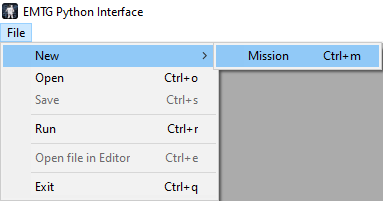
\includegraphics[width=0.7\linewidth]{../../shared_latex_inputs/images/pyemtg_file_new.png}
	\caption{EMTG File Menu}
\end{figure}
				
\noindent Once an EMTG mission is populated in the GUI, several tabs become visible to the user where they can alter values through several input fields (i.e. calanderCTRL pickers, text fields, check boxes, drop-down menus). 

\begin{figure}[H]
	\centering
	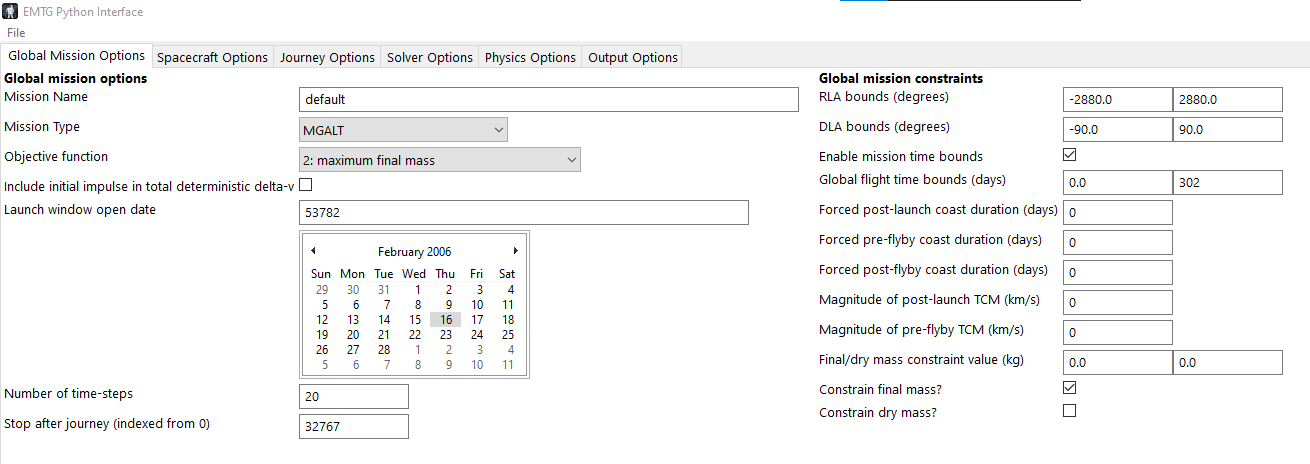
\includegraphics[width=0.7\linewidth]{../../shared_latex_inputs/images/pyemtg_global_options_tab.png}
	\caption{EMTG Global Mission Options Tab}
\end{figure}

\noindent The names of the tabs are as followed:
\begin{itemize}
	\item Global Mission Options
	\item Spacecraft Options
	\item Journey Options
	\item Solver Options
	\item Physics Options
	\item Output Options
\end{itemize}

\noindent The following are keyboard sequences that allow a user to navigate through the \ac{GUI} tabs:
\begin{itemize}
	\item Ctrl + Tab: Go to the next GUI Tab
	\item Ctrl + Shift + Tab: Go to the previous GUI Tab
	\item Shift + Tab: Go to a previous input field
	\item Tab: Go to the next input field
\end{itemize}

\noindent Once a user enters the calendarCTRL input field, the following keyboard sequences allow a user to select a date and navigate:
\begin{itemize}
	\item arrow keys: Move to a new day/Month/Year/Year-Range
	\item Tab: Exit calendar input field to next input field
	\item Shift+Tab: Exit calendar input field to previous input field
	\item Ctrl + up arrow: Zoom out upper calendar selection to be broader (e.g. going from month to year, year to year-range)
	\item Ctrl + down arrow: Zoom in upper calendar  selection to be narrower 
	\item Ctrl + left/right arrow: Move to next value of the upper calendar selection
\end{itemize}

%%%%%%%%%%%%%%%%%%%%%%%%
\section{PEATSA}
\label{sec:peatsa}
%%%%%%%%%%%%%%%%%%%%%%%%

%%%%%%%%%%%%%%%%%%%%%%%%
%\section{PEATSA}
%\label{sec:peatsa}
%%%%%%%%%%%%%%%%%%%%%%%%

\ac{PEATSA} is a set of Python scripts used to create and execute \ac{EMTG} trade studies. \ac{PEATSA} operates by taking an \ac{EMTG} options file (the ``base case''\footnote{nomenclature that may be unfamiliar to a non-\ac{PEATSA} user is written in quotes on first reference.}) and executing variations of some of those options. The user sets the different variations prior to exectution. For example, a user might vary the launch date, the launch vehicle, a gravity-assist sequence, and/or a maximum time of flight. One execution of all desired variations constitutes a ``\ac{PEATSA} iteration.'' At the end of each iteration, a user-defined objective function is evaluated for each \ac{EMTG} case, and this value is compared against the best objective function value achieved in any previous iteration for each \ac{EMTG} case. The \ac{EMTG} execution with the best value of the objective function for each case is saved, and information about the best execution for each case is written to a summary file.

\noindent For the next iteration, initial guesses for \ac{EMTG} cases are generated based on existing results from cases with similar option variations. For example, if the user is varying the launch date (i.e., the launch date is a trade parameter), then the user can allow a case to use an initial guess solution from another case (a ``neighbor'') as long as the launch dates of the two cases are within the vicinity of  \(\sim \)5 days of each other, and all other trade parameters are the same between the two cases. This process is called ``seeding'' or using one case to ``seed'' another. The idea behind seeding is that similar solutions are likely to exist between neighboring cases, so using a neighbor as a seed is likely to result in a feasible solution. In this way, a solution for a single case can turn into a ``family'' of solutions after a number of iterations as neighbor $i$ seeds neighbors $i+1$ and $i-1$ on iteration $j$, and then neighbor $i+1$ seeds neighbors $i$ and $i+2$ on iteration $j+1$. Note that in the preceding description, a neighbor that is used as a seed may also be seeded by a neighbor of its own. As a result, any new optimal solution can ``propagate'' to create a new solution family.

\noindent The remainder of this section decribes how to create, execute, and analyze the results of a \ac{PEATSA} run.

%%%%%%%%%%%%%%%%%%%%%%%%
\subsection{Creating a PEATSA Run}
\label{sec:creating_a_peatsa_run}
%%%%%%%%%%%%%%%%%%%%%%%%

%%%%%%%%%%%%%%%%%%%%%%%%
%\subsection{Creating a PEATSA Run}
%\label{sec:creating_a_peatsa_run}
%%%%%%%%%%%%%%%%%%%%%%%%

At the most fundamental level, three things are required to execute a \ac{PEATSA} run:

\begin{itemize}
	\item \ac{EMTG} options file: This is called the base case and must be able to produce a valid/feasible solution.
	\item \ac{PEATSA} options file: This is a Python file that specifies the options to be used when executing the run. This is also known as the ``trade study options file''.
	\item \ac{PEATSA} trade parameters file: This csv file sets the trade parameters of the \ac{PEATSA} run.
\end{itemize}

\noindent These three items are described in more detail in Sections~\ref{sec:peatsa_base_case}, \ref{sec:creating_the_peatsa_options_file}, \ref{sec:customizing_the_peatsa_options_file}, and \ref{sec:peatsa_trade_parameters_file}.

\subsubsection{The Base Case}
\label{sec:peatsa_base_case}

The base case is an \ac{EMTG} options file that can produce a feasible solution. The purpose of the base case is to set the default values of the options for an \ac{EMTG} run that \ac{PEATSA} will then systematically change in order to perform the trade study. Once a problem requiring a \ac{PEATSA} run is identified, the most common workflow is to use the PyEMTG \ac{GUI} to create the base case. In this pre-\ac{PEATSA} phase, it is beneficial but not absolutely necessary to find a feasible solution for the base case and set the initial guess for the base case to be that feasible solution.

\subsubsection{Creating the PEATSA Options File}
\label{sec:creating_the_peatsa_options_file}

The \ac{PEATSA} options file is a Python file that specifies the options to be used when executing the \ac{PEATSA} run. The \ac{PEATSA} options file uses Python syntax, but it is not actually an end-to-end script or function. Instead, it is a sequence of variable assignments that is evaluated by \ac{PEATSA}.

\noindent A new \ac{PEATSA} options file is created by either duplicating and then modifying an existing \ac{PEATSA} options file or by using the PEATSA\_script\_generator.py utility script in \\ \textbf{\textless EMTG\_root\_dir\textgreater}/PyEMTG/PEATSA, where \textbf{\textless EMTG\_root\_dir\textgreater} is the top level directory of EMTG that has the /bin/ directory as a sub-directory. To create a new \ac{PEATSA} options file, execute the PEATSA\_script\_generator.py script in Python. The script prompts the user to answer a series of questions in order to create the desired \ac{PEATSA} options file for the run. (Some elements here are not described in detail yet; information will be added later, but the current contents are enough to create a new \ac{PEATSA} run.)

\begin{enumerate}
	\item \texttt{\# How should PEATSA start? ... Enter start\_type = }
	\begin{itemize}
		\item \texttt{Fresh}. Used when starting a new \ac{PEATSA} run. This is the most commonly used option.
		\item \texttt{Warm}
		\item \texttt{Hot}
	\end{itemize}
	\item \texttt{\# What type of PEATSA run is this? ... Enter PEATSA\_type = }
	\begin{itemize}
		\item \texttt{0}.
		\item \texttt{1}.
		\item \texttt{2}. A trade study. This is the option used to systematically vary \ac{EMTG} options to perform a trade study.
		\item \texttt{3}.
		\item \texttt{4}.
		\item \texttt{5}.
	\end{itemize}
	\item \texttt{\# What is the objective type? ... Enter objective\_type = }
	\begin{itemize}
		\item \texttt{0}. A new feasible \ac{EMTG} solution is considered superior to an old solution if the new solution's \ac{PEATSA} objective function is better than the old solution's \ac{PEATSA} objective function.
		\item \texttt{1}.
	\end{itemize}
	\item \texttt{\# Should the default plots be generated? ... Enter generate\_default\_plots = }
	\begin{itemize}
		\item \texttt{0}. Do not generate default plots. The default plots do not currently work, so this option should be chosen.
		\item \texttt{1}.
	\end{itemize}
	\item \texttt{Enter filename: }
	\begin{itemize}
		\item Full path to and name of file in which to write the new \ac{PEATSA} script. Filename should end with .py.
	\end{itemize}
\end{enumerate}

\noindent After the execution of PEATSA\_script\_generator.py, the filename entered by the user is populated with options that the user sets to customize the \ac{PEATSA} run. 

\subsubsection{Customizing the PEATSA Options File}
\label{sec:customizing_the_peatsa_options_file}

A \ac{PEATSA} options file created by executing PEATSA\_script\_generator.py is not ready to be run. Some options have valid default values that the user may wish to change, while other options \emph{must} be set by the user prior to execution.  The listing of options below are a subset of the options available that are important to understand. Refer to the comments in the option file for information on all options available.

\begin{itemize}
	\item run\_name \\ Directory for \ac{PEATSA} to create, which it populates with the files it generates. This option sets the name of that directory. Do not use a file path here.
	\item working\_directory \\ Full directory path to the location in which the run\_name directory will be created. The path does not need to end with a file separator.
	\item nCores \\ A two element array associated with how \ac{PEATSA} will split up its processes. Leave the first element of the tuple set to 'local'. Set the second element of the tuple to the number of parallel processes you want \ac{PEATSA} to use.
	\item emtg\_root\_directory \\  Full path to the \ac{EMTG} bin directory.
	\item if\_run\_cases \\ Set this to 1 to execute the \ac{EMTG} cases.
	\item trade\_study\_options\_files \\ The list is populated with 2-element tuples. The first element of each tuple is a string containing the full path to a trade parameter csv, and the second element is an integer specifying the type of the trade parameter csv. (See Section~\ref{sec:peatsa_trade_parameters_file}.)
	\item killtime \\ This sets a maximum time in seconds that an \ac{EMTG} case is allowed to run before \ac{PEATSA} kills the process. The comments in the options file give best practices for setting this value.
	\item objective\_formula \\ This sets the \ac{PEATSA} objective value; that is, how \ac{PEATSA} decides if one \ac{EMTG} run is better than another. The formula must be a function of data that is obtainable from a PyEMTG Mission object and MissionOptions object for a given \ac{EMTG} run.\footnote{The Mission object gives information that can only be evaluated \emph{after} an \ac{EMTG} case is executed, while a MissionOptions object gives information that is known \emph{prior} to \ac{EMTG} case execution.} These objects are accessed via `M.' and `MO.', respectively (e.g., `M.total\_deterministic\_deltav' gives the total deterministic $\Delta v$ of a solution). \\ Note that this objective value does not have to be the same as the objective function for a single \ac{EMTG} run.
	\item max\_or\_min \\ Set whether the objective\_formula should be maximized or minimized.
	\item peatsa\_goal\_objective \\ Set appropriately based on the objective\_formula. (See the comments in the options file give best practices for setting this value.)
	\item fingerprint \\ The list of strings in the fingerprint defines a unique \ac{EMTG} case. A good starting point is to make the fingerprint a list of the trade parameter column headers (See Section~\ref{sec:peatsa_trade_parameters_file}). \\ Note: Disregard the ``Do not put any formulas that are already in the seed\_criteria list'' sentence in the option file comments for this option. It is WRONG.
	\item seed\_folders \\ Seeds refers to \ac{EMTG} solution files (*.emtg files) that can be used as initial guesses for \ac{EMTG} cases generated by \ac{PEATSA}. A seed folder contains one or more of these solution files. The seed\_folders option is a list of tuples. The first element of the tuple is an integer describing the type of the folder.  The second element is a string containing the full path to the seed folder. (See the comments in the options file for additional details.)
	\item seed\_from\_seed\_folders\_on\_fresh\_start \\ Set whether an external seed folder should be used before the first \ac{PEATSA} iteration. The default value is False, but it is usually more likely that a user wants to set it to True if using seed folders.
	\item seed\_from\_cases\_that\_havent\_met\_target \\ Set whether cases that don't meet the \ac{PEATSA} goal criteria can be used as a seed in another case. The default value if 0, but it is likely that a user wants to set it to 1.
	\item seed\_criteria \\ This option describes how an existing \ac{EMTG} solution may be used as an initial guess for a new \ac{EMTG} case with a similar, but not necessarily identical, set of trade parameters. seed\_criteria is a list of 4-element tuples. The first element is a string that is the criterion to be compared between an \ac{EMTG} case and a potential seed case. This should be a trade parameter as defined in the trade parameters csv file. (See Section~\ref{sec:peatsa_trade_parameters_file}.) The second element is a real number that is the maximum negative seed range. In other words, when evaluating a potential seed case, how much less than the current case can the seed criterion be for the seed case and still be considered a potential seed? The third element is a real number that is the maximum positive seed range. In other words, when evaluating a potential seed case, how much greater than the current case can the seed criterion be for the seed case and still be considered a potential seed? The fourth element is an integer and is the seed selection criterion. The choices are described fully in the comments of the \ac{PEATSA} options file. Additional notes about seed\_criteria:
	\begin{itemize}
		\item In order for case A to be a potential seed for case B, case A's fingerprint must be identical to case B's fingerprint except for the value of the seed\_criteria element under evaluation.
		\item The elements of the seed\_criteria list are evaluated one at a time. In other words, there is no ``and'' or ``or'' logic. Each list element creates seeded cases independently of the others.
	\end{itemize}
	\item override\_options \\ A list of two-element tuples used to set \ac{EMTG} options that are different from the base case but are not trade parameters. The first element of a tuple is a logical condition that is evaluated to see if that specific override should be applied. The second element of a tuple is the formula for that specific override option, of the form `option = value'. A PyEMTG MissionOptions object is accessed via `MO'. If a string is required as part of the tuple, then use single quotes to enclose the entire tuple and double quotes to enclose the string element. 
	
	See the following examples of the most commonly used override options:
	\begin{itemize}
		\item (`1', `MO.HardwarePath = ``/path/to/HardwareModels/''')
		\item (`1', `MO.universe\_folder = ``/path/to/universe/''')
		\item (`1', `MO.MBH\_max\_run\_time = 120') \# or some other value
		\item (`1', `MO.snopt\_max\_run\_time = 10') \# or some other value
		\item (`1', `MO.quiet\_basinhopping = 1') \# or some other value
		\item (`1', `MO.short\_output\_file\_names = 1') \# or some other value
	\end{itemize}
	\item extra\_csv\_column\_definitions \\ (See Section~\ref{sec:peatsa_outputs}) After each \ac{PEATSA} iteration, a summary csv file is created. There is a row for each unique \ac{EMTG} case, as defined by the \ac{PEATSA} fingerprint. There are columns with data about each case. The extra\_csv\_column\_definitions is used to define columns of the summary csv with data that the user is interested in for that particular \ac{PEATSA} run. A column is added by adding a two-element tuple to the extra\_csv\_column\_definitions. The first element is a string defining the column header. The second element is a string that may be evaluated for a given \ac{EMTG} run. Data must be obtainable from a PyEMTG Mission object and MissionOptions object for a given \ac{EMTG} run. These objects are accessed via `M.' and `MO.', respectively. Both Mission and MissionOptions have a `Journeys' list: a list of Journey objects for Mission and a list of JourneyOptions objects for MissionOptions. In addition, each Journey object has a list of missionevents objects. 
	
	See the following for examples of useful csv columns to include:
	\begin{itemize}
		\item (`LaunchVehicle', `MO.LaunchVehicleKey')
		\item (`C3 (km2/s2)', `M.Journeys[0].missionevents[0].C3')
		\item (`TotalDeltaV (km/s)', `M.total\_deterministic\_deltav')
		\item (`DryMass (kg)', `M.spacecraft\_dry\_mass')
		\item (`TotalFlightTime (years)', `(M.Journeys[-1].missionevents[-1].JulianDate - \\M.Journeys[0].missionevents[0].JulianDate)/365.25')
		\item (`Flyby 0 GregorianDate (TDB)', \\`M.Journeys[0].getMGAPhaseUnpoweredFlyby(0).GregorianDate')
		\item (`Phase 0 Arrival Sun Periapse Distance (au)', \\`M.Journeys[0].GetBoundaryConstraintOutputValueByName\\(``j0p0MGAnDSMsEphemerisPeggedFlybyIn periapse distance'', ``float'') / 1.49597870691e+8')
	\end{itemize}
\end{itemize}

\subsubsection{The PEATSA Trade Parameters File}
\label{sec:peatsa_trade_parameters_file}

The \ac{PEATSA} trade parameters file contains the path to the base case and sets the trade parameters and their values for the \ac{PEATSA} run. The trade parameters file is a csv file, and it is recommended to view and edit the file using Microsoft Excel or another spreadsheet tool rather than a text editor.

\noindent The first row of the csv contains the full path to the directory containing the base case. The path does not need to end with a file seperator. The path does not contain the name of the actual \ac{EMTG} options file itself --- just the path to the directory in which it resides.

\noindent The second row of the csv contains the name of the \ac{EMTG} options file for the base case. This file must be inside the directory specified on the first row.

\noindent The third row of the csv lists, as comma-seperated values, the names of the \ac{EMTG} options that are trade parameters. The trade parameters are accessed by accessing attributes of the PyEMTG MissionOptions class. Here, a MissionOptions instance for the base case is accessed via `MO'. For example, if it is desired to set the maximum total time of flight as a trade parameter, an element of row 3 would be `MO.total\_flight\_time\_bounds[1]'. In this example, the index 1 is used because the total\_flight\_time\_bounds attribute is a two-element list containing the lower bound and upper bound of the total time of flight. Another list attribute that is frequently used is `Journeys', which is a list of JourneyOptions objects, one for each Journey of the Mission. For example, `MO.Journeys[1].duty\_cycle' would make the duty cycle of Journey index 1 (the indexing starts from 0) a trade parameter.

\noindent Rows four and below list the values of the trade parameters. The desired values for a given trade parameter are listed in the column in which the name of that trade parameter was written in row 3. Three different formats are available.

\noindent The following are examples of different valid types of trade parameter files in \\ \textbf{\textless EMTG\_root\_dir\textgreater}/PyEMTG/PEATSA:

\begin{itemize}
	\item Type 0.
	\begin{itemize}
		\item Trade all values for a given trade parameter individually against the base-case values of all other trade parameters.
		\item The number of rows for each column may be different.
		\item The total number of cases is equal to the sum of the number of rows of each column, starting with row 4.
		\item There is an example in \textbf{\textless EMTG\_root\_dir\textgreater}/PyEMTG/PEATSA/opt\_file\_type\_zero.csv.
	\end{itemize}
	\item Type 1.
	\begin{itemize}
		\item Trade all values of each variable against all values of all other variables. An \ac{EMTG} case is created for every permuation of the values listed in rows 4 and below.
		\item The number of rows for each column may be different.
		\item The total number of cases is equal to the product of the number of rows of each column, starting with row 4.
		\item There is an example in \textbf{\textless EMTG\_root\_dir\textgreater}/PyEMTG/PEATSA/opt\_file\_type\_one.csv.
	\end{itemize}
	\item Type 2.
	\begin{itemize}
		\item The columns of each row represent a set of trade parameters that defines an \ac{EMTG} case to be run.
		\item The number of rows for each column must be the same.
		\item The total number of cases is equal to the number of rows, starting with row 4.
		\item There is an example in \textbf{\textless EMTG\_root\_dir\textgreater}/PyEMTG/PEATSA/opt\_file\_type\_two.csv.
	\end{itemize}
\end{itemize}

%%%%%%%%%%%%%%%%%%%%%%%%
\subsection{Executing PEATSA}
\label{sec:executing_peatsa}
%%%%%%%%%%%%%%%%%%%%%%%%

%\subsection{Executing \ac{PEATSA}}
%\label{sec:executing_peatsa}

Once the files required to set up a PEATSA run has been created, the command-line command to execute a PEATSA run is (all on one line):

\setlength\parindent{-15pt} \verb|nohup python path/to/PEATSA.py /path/to/trade_study_file.py > /path/to/peatsa.out 2>&1 &|

\noindent The following is a breakdown of the different elements of this command:

\begin{itemize}
	\item \verb|nohup|: Ignore the hangup signal so that the process does not stop if the user logs out or is diconnected.
	\item \verb|python path/to/PEATSA.py /path/to/trade_study_file.py|: Use python to execute \\ PEATSA.py with trade\_study\_file.py as a command-line argument.
	\item \verb|> /path/to/peatsa.out 2>&1|: Redirect standard output and standard error to peatsa.out. \ac{PEATSA} writes output to this file, so the user can monitor the progress of a \ac{PEATSA} run by examining the contents of this file. The user can also see if a \ac{PEATSA} run has died unexpectedly by examining the contents of this file.
	\item \verb|&|: Run in the background.
\end{itemize}	

%%%%%%%%%%%%%%%%%%%%%%%%
\subsection{PEATSA Outputs}
\label{sec:peatsa_outputs}
%%%%%%%%%%%%%%%%%%%%%%%%

%\subsection{\ac{PEATSA} Outputs}
%\label{sec:peatsa_outputs}

When a \ac{PEATSA} run is initiated, information is output to a number of places:

\begin{itemize}
	\item Standard output and standard error messages are written to the file specified at the command line in the \ac{PEATSA} execution call. (See Section~\ref{sec:executing_peatsa}.)
	\item Logging information is written to the file specified using the logfile option in the \ac{PEATSA} options file.
	\item A new directory is created in the location specified by the run\_name and working\_directory options in the \ac{PEATSA} options file.
\end{itemize}

\noindent The contents of the new directory created by \ac{PEATSA} are as followed:

\begin{itemize}
	\item docs/. This directory contains two types of files:
	\begin{itemize}
		\item PEATSAhistory.csv. Only a single file of this type is created, and that file is overwritten at the end of each \ac{PEATSA} iteration. This file contains extremely basic information about each \ac{PEATSA} iteration, such as how many \ac{EMTG} runs were executed, how many \ac{EMTG} runs found a feasible solution, and how many unique \ac{PEATSA} cases found a better value of the \ac{PEATSA} objective function in a given iteration. This information is useful for knowing if a \ac{PEATSA} run should be stopped, tweaked, and re-started (e.g., if no cases are producing feasible results) or if a \ac{PEATSA} run should be ended (e.g., because no cases have found more optimal solutions in several iterations).
		\item IterationX.csv, where X is the iteration index, starting with 0. A new file of this type is created at the end of each \ac{PEATSA} iteration. Each file gives information about the most optimal case that has been found up through that iteration for each unique \ac{PEATSA} case, as defined by the fingerprint. (See Section~\ref{sec:customizing_the_peatsa_options_file}.) Some information is given by default, such as the file path to the *.emtg and *.emtgopt file, and the feasibility index. Additional information is added by adding tuples to the extra\_csv\_column\_definitions list in the \ac{PEATSA} options file. (See Section~\ref{sec:customizing_the_peatsa_options_file}.)
	\end{itemize}
	\item results/. This directory contains subdirectories in which the output *.emtg, *.emtgopt, and *.emtg\_spacecraftopt files produced for each \ac{PEATSA} iteration are written.
	\item cases/. This directory contains subdirectories in which the input *.emtgopt files produced for each \ac{PEATSA} iteration are written.
	\item images/. This directory contains plots generated by the \ac{PEATSA} iterations.
	\item HardwareModels/. This directory contains \ac{EMTG} hardware files needed for each \ac{PEATSA} iteration (e.g., .emtg\_spacecraftopt).
	\item PEATSA\_iteration\_kill\_file.DEATH. The contents of the text file may be edited to end a \ac{PEATSA} iteration or an entire \ac{PEATSA} run. See the comments in the file for more details.
	\item PEATSA\_MidBake\_Options.py. The file is similar to a \ac{PEATSA} options file, but it specifically only has options that a user is allowed to change from iteration to iteration of a \ac{PEATSA} run.
	\item PEATSA\_ExecutedOptions.py. This file holds the values of the \ac{PEATSA} options used to kick off the \ac{PEATSA} run.
\end{itemize}

%%%%%%%%%%%%%%%%%%%%%%%%
\subsection{PEATSA Tips and Tricks}
\label{sec:peatsa_tips_and_tricks}
%%%%%%%%%%%%%%%%%%%%%%%%

%\subsection{\ac{PEATSA} Tips and Tricks}
%\label{sec:peatsa_tips_and_tricks}

\begin{itemize}
	\item Use the Linux `top' command to see what processes are currently active on a server. This can be used to make sure that a \ac{PEATSA} run is currently executing. This can also be used prior to kicking off a \ac{PEATSA} run to make sure that someone else is not already using the server.
	\item Use the Linux `tail' command to observe live updates to the contents of a logfile or case output.
	\item The python script \textbf{\textless EMTG\_root\_dir\textgreater}/PyEMTG/PEATSA/grab\_best\_peatsa\_results.py is used to take the full	results of a \ac{PEATSA} run and extract only the feasible case with the best value of the objective function for each unique trade case. This can be a great space-saver because it can allow the user to delete a full \ac{PEATSA} run without losing the best solutions. If desired, the best results can be used as seed cases for a new \ac{PEATSA} run to ``continue'' an old run, too. However, be careful, because this script does not save summary csv files, etc.
\end{itemize}



\end{document}